%%%%%%%%%%%%%%%%%%%%%%%%%%%%%%%%%%%%%%%%%%%%%%%%%%%%%%%%%%%%%%%%%%%%%%%%%%%%%%%%%%
\begin{frame}[fragile]\frametitle{}
\begin{center}
{\Large Rasa Chatbot Deployment: Slack}

\end{center}
\end{frame}

%%%%%%%%%%%%%%%%%%%%%%%%%%%%%%%%%%%%%%%%%%%%%%%%%%%%%%%%%%%
\begin{frame}[fragile]\frametitle{What is Slack?}
\begin{itemize}
\item A chat room for all your company communications.
\item Essentially a replacement for your emails
\item Organizes into Workshapces (Groups)
\item Within Workspaces you can have channels (Projects) with different people.
\item Slack integrates with a host of other apps so you can manage your entire workflow through one platform
\end{itemize}

\end{frame}

%%%%%%%%%%%%%%%%%%%%%%%%%%%%%%%%%%%%%%%%%%%%%%%%%%%%%%%%%%%
\begin{frame}[fragile]\frametitle{Slack Account Creation}
\begin{itemize}
\item First, create Slack Account with a Workspace.
\item Create a new Workspace,https://slack.com/create give email, verify it
\item Name of your company ``DataHacksConf2019'', thats the workspace name.
\item Project name ``rasachatbot'', thats the channel name.
\end{itemize}

\end{frame}

%%%%%%%%%%%%%%%%%%%%%%%%%%%%%%%%%%%%%%%%%%%%%%%%%%%%%%%%%%%
\begin{frame}[fragile]\frametitle{Slack App}
\begin{itemize}
\item Then, create a Slack App. WIthin Workshpace, you can have Apps apart from Channels.
\item Visit https://api.slack.com/
\item Create a Slack app in ``RasaChatBotDemo'', 
\item Select ``DataHacksConf2019'' as Workspace
\end{itemize}

\begin{center}
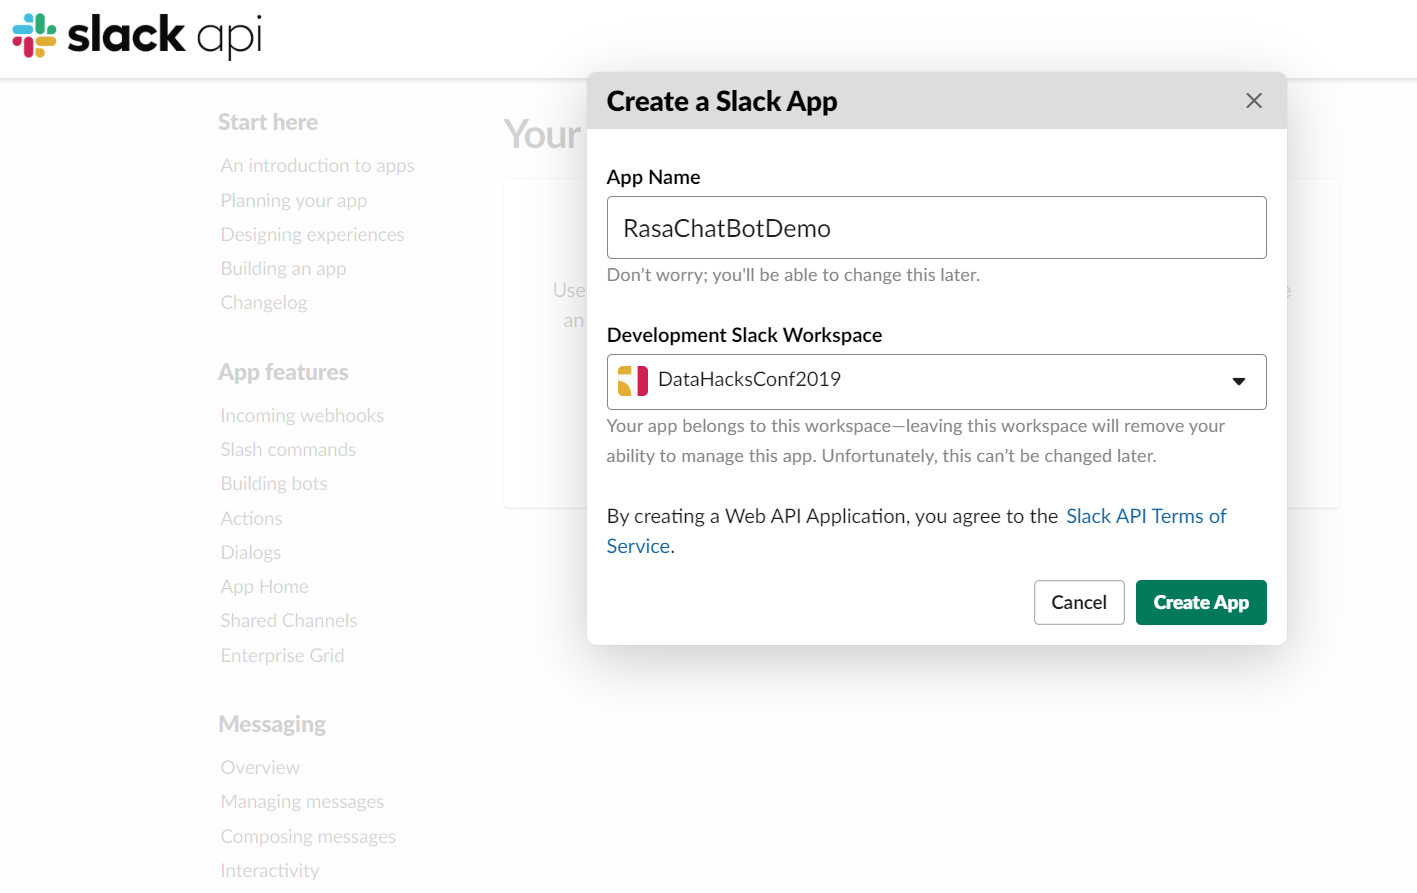
\includegraphics[width=0.7\linewidth]{rasa27}
\end{center}
\end{frame}

%%%%%%%%%%%%%%%%%%%%%%%%%%%%%%%%%%%%%%%%%%%%%%%%%%%%%%%%%%%
\begin{frame}[fragile]\frametitle{Slack App}
\begin{itemize}
\item In ``Add features and functionalities'' panel, select ``Bots'' tab.
\item Also, available on the left hand menu, you will see ``Features'', Select ``Bots Users''
\item ``Add a Bot user'' with defaults
\item Select ``OAuth \& Permissions'', review if all ok. No changes may be needed here.
\item Click ``Basic Information' on left hand menu, you should see both ``Bots'' and ``Permissions'' tabs selected.
\end{itemize}

\begin{center}
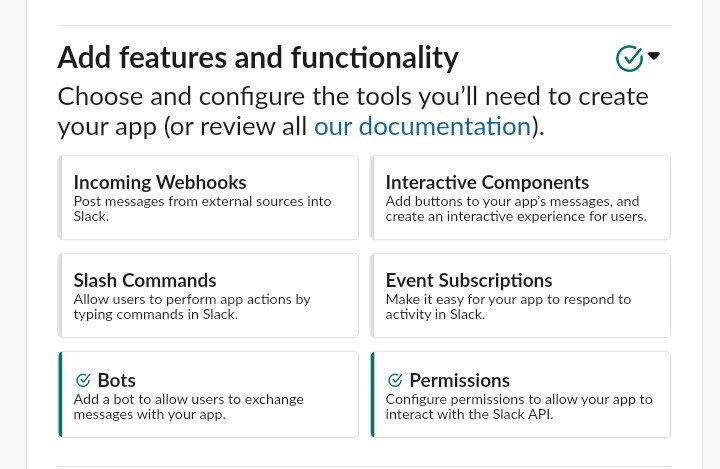
\includegraphics[width=0.7\linewidth]{rasa28}
\end{center}
\end{frame}

%%%%%%%%%%%%%%%%%%%%%%%%%%%%%%%%%%%%%%%%%%%%%%%%%%%%%%%%%%%
\begin{frame}[fragile]\frametitle{Slack App}
\begin{itemize}
\item Scroll to Display Information and add more about our bot like a picture, a description and a background colour.
\item Picture needs to be specific quality as shown in the picture below.
\item Save all changes (button below)
\item ``Install App Workspace''. Authorize (``Allow'') it and we have our app ready and integrated into the workplace.
\end{itemize}

\begin{center}
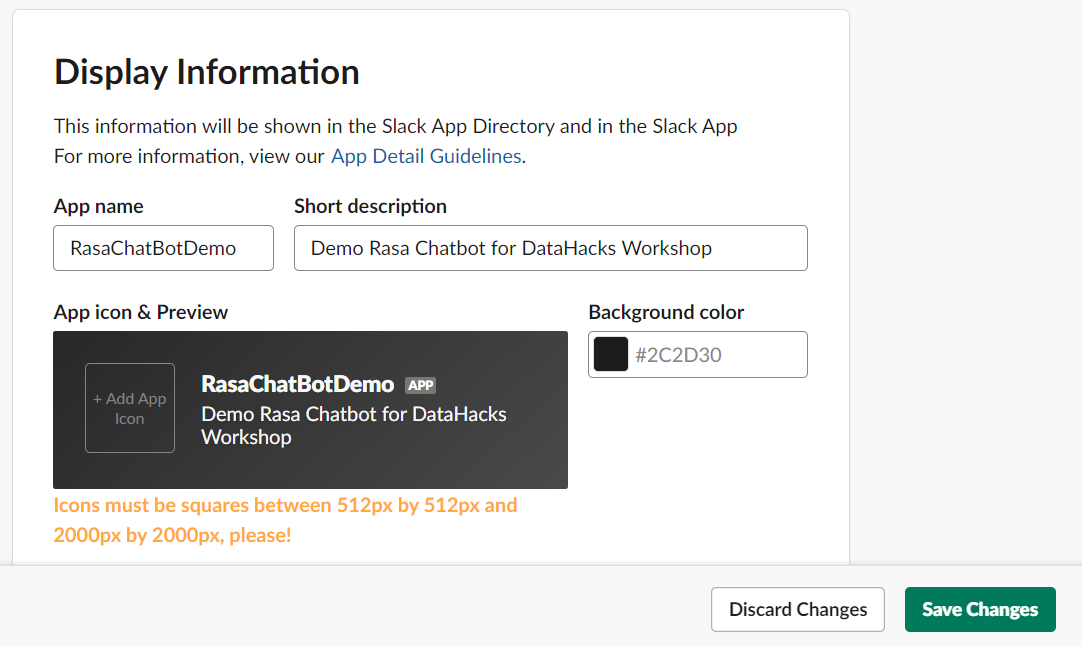
\includegraphics[width=0.5\linewidth]{rasa29}
\end{center}
\end{frame}

%%%%%%%%%%%%%%%%%%%%%%%%%%%%%%%%%%%%%%%%%%%%%%%%%%%%%%%%%%%
\begin{frame}[fragile]\frametitle{Ngrok}
\begin{itemize}
\item Ngrok is a multiplatform tunnelling.
\item Gives your machine a domain name so that Facebook, Slack, etc. know where to send messages to reach your local machine.
\item Download ngrok from https://ngrok.com/download 	
\item Extrtact the zip to the exe. Its a command line application.
\item Now ,Start it with which port we want to expose to the public internet : \lstinline| ./ngrok http 5004|
\end{itemize}

\begin{center}
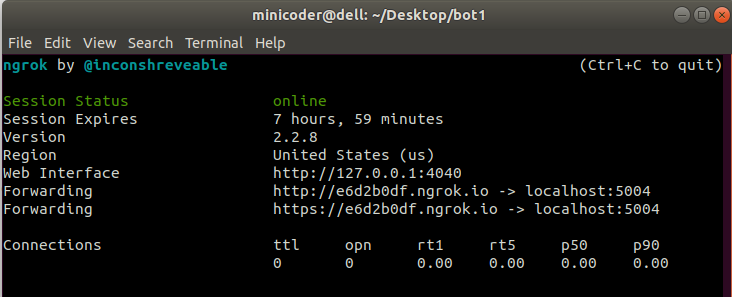
\includegraphics[width=0.5\linewidth]{rasa30}
\end{center}
\end{frame}

%%%%%%%%%%%%%%%%%%%%%%%%%%%%%%%%%%%%%%%%%%%%%%%%%%%%%%%%%%%
\begin{frame}[fragile]\frametitle{Deploy Chatbot on Slack}
Create ``run.py''
\begin{lstlisting}
from rasa_core.channels.slack import SlackInput
from rasa_core.agent import Agent
from rasa_core.interpreter import RegexInterpreter
from rasa_core.interpreter import RasaNLUInterpreter
nlu_interpreter = RasaNLUInterpreter('./models/nlu/default/current')
agent = Agent.load('./models/dialogue', interpreter = nlu_interpreter)
input_channel = SlackInput(
        slack_token="******************************"
        # this is the `bot_user_o_auth_access_token`
        #slack_channel="YOUR_SLACK_CHANNEL"
            # the name of your channel to which the bot posts (optional)
    )
# set serve_forever=True if you want to keep the server running
s = agent.handle_channels([input_channel], 5004, serve_forever=True)
\end{lstlisting}

\end{frame}

%%%%%%%%%%%%%%%%%%%%%%%%%%%%%%%%%%%%%%%%%%%%%%%%%%%%%%%%%%%
\begin{frame}[fragile]\frametitle{Deploy Chatbot on Slack}
The Slack Token can be optained from


\begin{center}
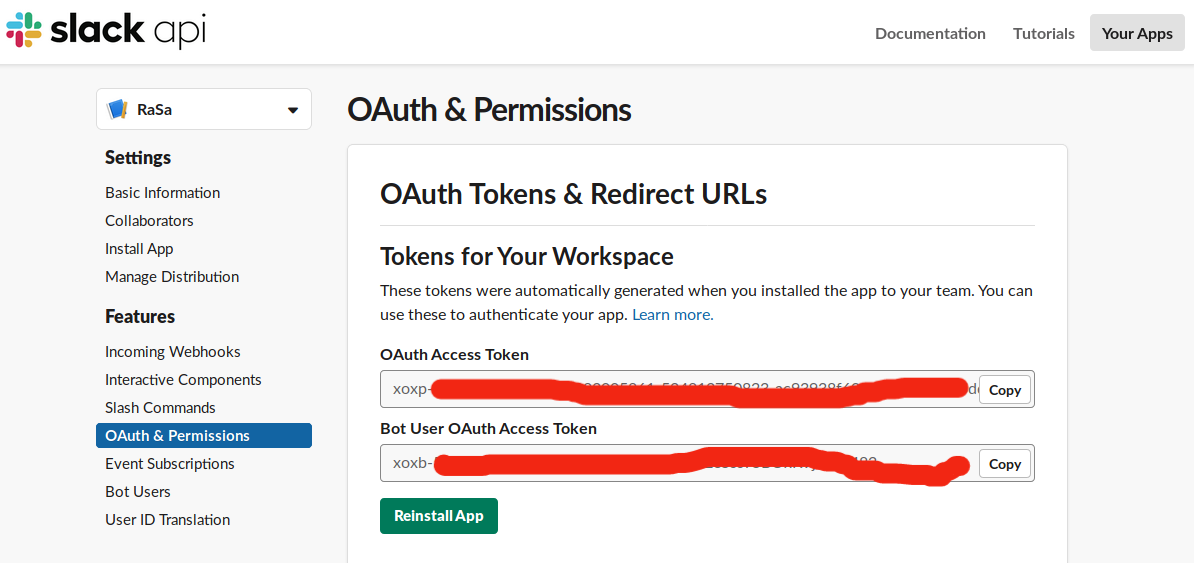
\includegraphics[width=0.8\linewidth]{rasa31}
\end{center}
\end{frame}


%%%%%%%%%%%%%%%%%%%%%%%%%%%%%%%%%%%%%%%%%%%%%%%%%%%%%%%%%%%
\begin{frame}[fragile]\frametitle{Deployment}
\begin{itemize}
\item Start the Agent by running run.py file .
\item Start the ngrok on port 5004 and grab your ngrok\_url.
\item Provide the ngrok url to ``Event Subscriptions'' page of the Slack configuration. Wait for it to be verified.
\end{itemize}

\begin{center}
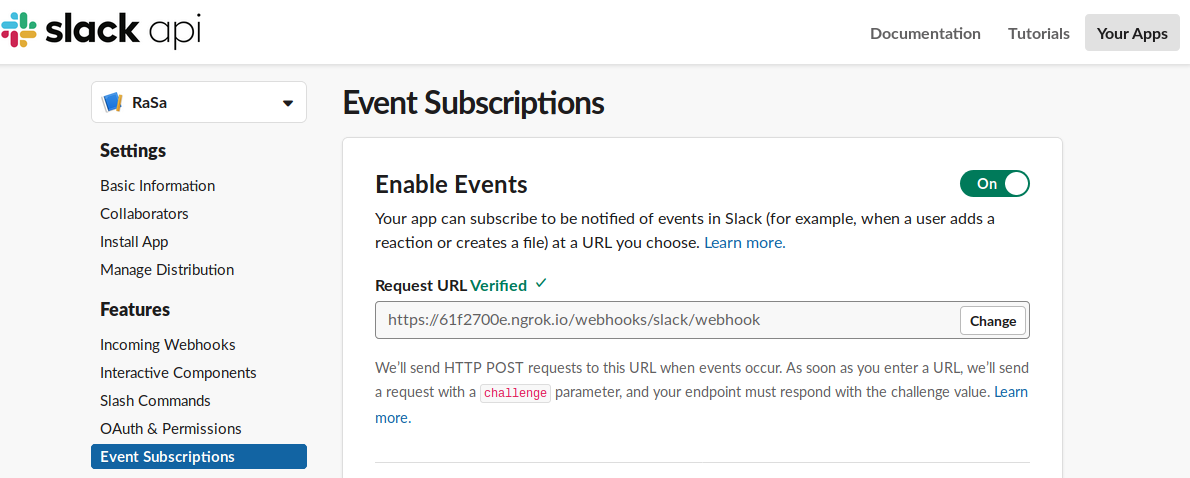
\includegraphics[width=0.8\linewidth]{rasa32}
\end{center}
\end{frame}


%%%%%%%%%%%%%%%%%%%%%%%%%%%%%%%%%%%%%%%%%%%%%%%%%%%%%%%%%%%
\begin{frame}[fragile]\frametitle{Deployment}
\begin{itemize}
\item Subscribe to some workplace events like:
\item ``app\_mention'' so that our bot responds when someone mentions it by name
\item ``message\_im'' which allows the user to send direct messages to the bot.
\item Save your all work.
\end{itemize}

\begin{center}
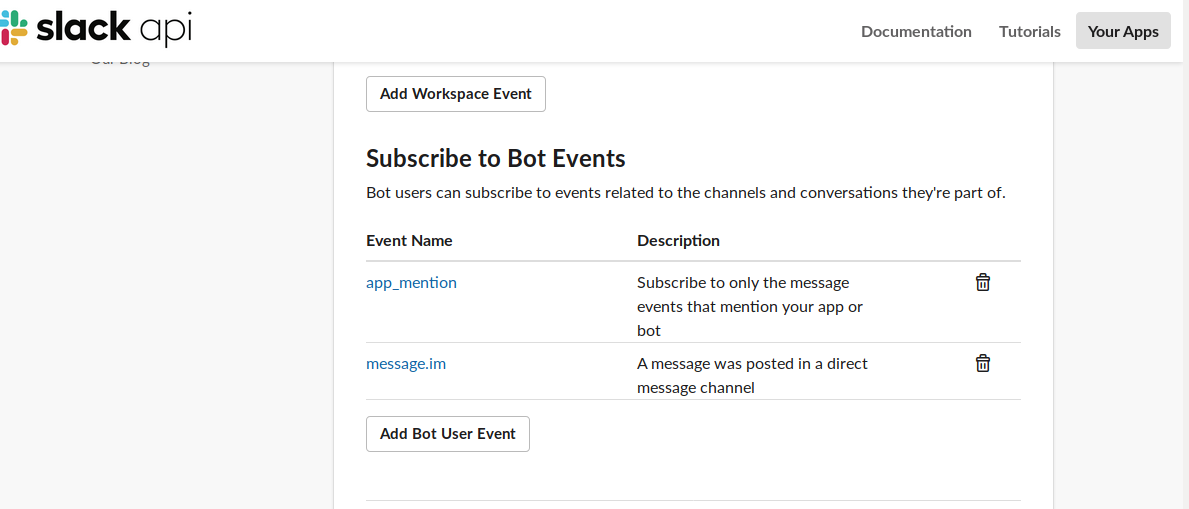
\includegraphics[width=0.7\linewidth]{rasa33}
\end{center}
\end{frame}

%%%%%%%%%%%%%%%%%%%%%%%%%%%%%%%%%%%%%%%%%%%%%%%%%%%%%%%%%%
\begin{frame}[fragile]\frametitle{Start chatting }
\begin{itemize}
\item Save your all work.
\item Now that everything is set up, you can just go to your Slack workspace and start chatting with your bot.
\item  Ensure the custom actions server is running (if you have custom actions)
\item Ensure ngrok is running on port 5004
\end{itemize}

\begin{center}
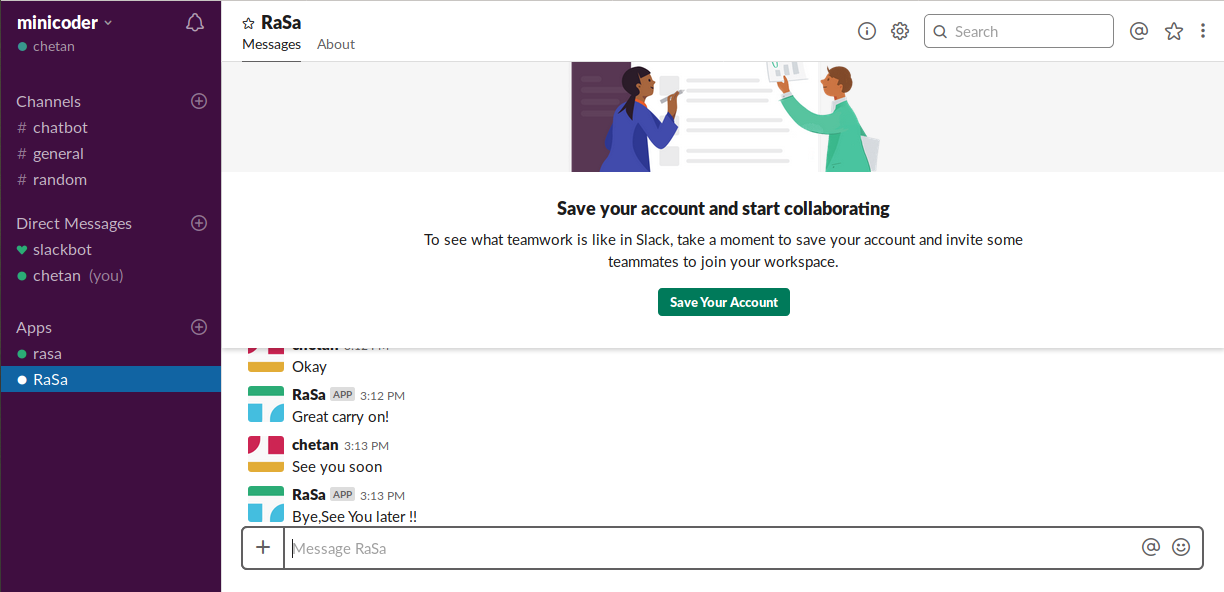
\includegraphics[width=0.5\linewidth]{rasa34}
\end{center}

Yup !! we Done
\end{frame}

%%%%%%%%%%%%%%%%%%%%%%%%%%%%%%%%%%%%%%%%%%%%%%%%%%%%%%%%%%%
\begin{frame}[fragile]\frametitle{What's Next?}
How these modules work? 

Can dig deep, to find what different integrations are available \ldots

And build one \ldots

\end{frame}
